% The architecture figure of the methods paper, written by scripts/paper-methods-figure.py
% from the same coordinates as site/public/paper/methods/figure-1.svg. Do not edit by hand.
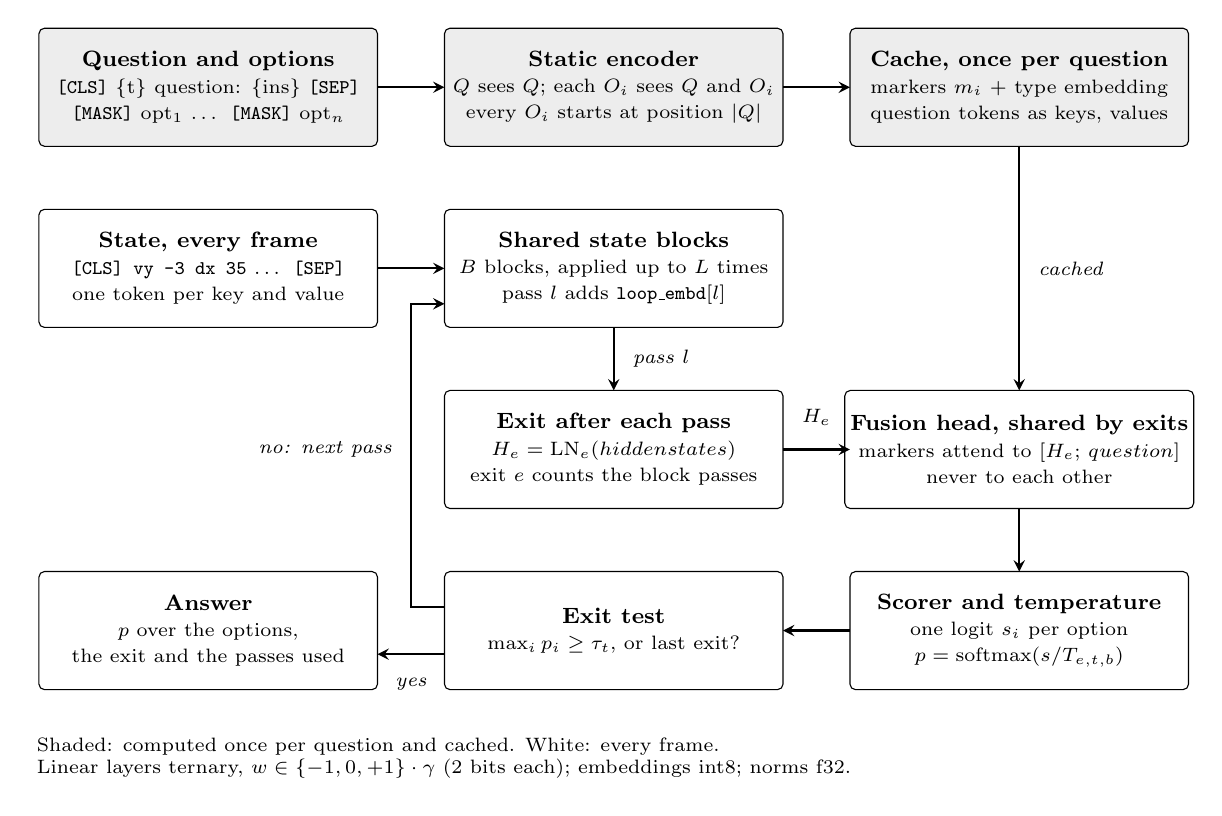
\begin{tikzpicture}[x=1cm,y=1cm,>=stealth,font=\footnotesize,box/.style={draw,rounded corners=2pt,minimum width=4.30cm,minimum height=1.50cm,align=center,inner sep=2pt}]
\node[box,fill=black!7] (in_q) at (2.30,8.50) {\textbf{Question and options}\\{\scriptsize \texttt{[CLS]} \{t\} question: \{ins\} \texttt{[SEP]}}\\{\scriptsize \texttt{[MASK]} opt$_1$ \ldots{} \texttt{[MASK]} opt$_n$}};
\node[box,fill=black!7] (static) at (7.45,8.50) {\textbf{Static encoder}\\{\scriptsize $Q$ sees $Q$; each $O_i$ sees $Q$ and $O_i$}\\{\scriptsize every $O_i$ starts at position $|Q|$}};
\node[box,fill=black!7] (cache) at (12.60,8.50) {\textbf{Cache, once per question}\\{\scriptsize markers $m_i$ + type embedding}\\{\scriptsize question tokens as keys, values}};
\node[box] (in_s) at (2.30,6.20) {\textbf{State, every frame}\\{\scriptsize \texttt{[CLS] vy -3 dx 35} \ldots{} \texttt{[SEP]}}\\{\scriptsize one token per key and value}};
\node[box] (loop) at (7.45,6.20) {\textbf{Shared state blocks}\\{\scriptsize $B$ blocks, applied up to $L$ times}\\{\scriptsize pass $l$ adds \texttt{loop\_embd}$[l]$}};
\node[box] (exit) at (7.45,3.90) {\textbf{Exit after each pass}\\{\scriptsize $H_e = \mathrm{LN}_e(\text{hidden states})$}\\{\scriptsize exit $e$ counts the block passes}};
\node[box] (fusion) at (12.60,3.90) {\textbf{Fusion head, shared by exits}\\{\scriptsize markers attend to $[H_e;\,\text{question}]$}\\{\scriptsize never to each other}};
\node[box] (score) at (12.60,1.60) {\textbf{Scorer and temperature}\\{\scriptsize one logit $s_i$ per option}\\{\scriptsize $p = \mathrm{softmax}(s / T_{e,t,b})$}};
\node[box] (test) at (7.45,1.60) {\textbf{Exit test}\\{\scriptsize $\max_i p_i \geq \tau_t$, or last exit?}};
\node[box] (answer) at (2.30,1.60) {\textbf{Answer}\\{\scriptsize $p$ over the options,}\\{\scriptsize the exit and the passes used}};
\draw[->,thick] (4.450,8.500) -- (5.300,8.500);
\draw[->,thick] (9.600,8.500) -- (10.450,8.500);
\draw[->,thick] (12.600,7.750) -- (12.600,4.650);
\node[anchor=west,font=\scriptsize\itshape] at (12.720,6.200) {cached};
\draw[->,thick] (4.450,6.200) -- (5.300,6.200);
\draw[->,thick] (7.450,5.450) -- (7.450,4.650);
\node[anchor=west,font=\scriptsize\itshape] at (7.570,5.050) {pass $l$};
\draw[->,thick] (9.600,3.900) -- (10.450,3.900);
\node[anchor=south,font=\scriptsize\itshape] at (10.025,4.080) {$H_e$};
\draw[->,thick] (12.600,3.150) -- (12.600,2.350);
\draw[->,thick] (10.450,1.600) -- (9.600,1.600);
\draw[->,thick] (5.300,1.300) -- (4.450,1.300);
\node[anchor=north,font=\scriptsize\itshape] at (4.875,1.120) {yes};
\draw[->,thick] (5.300,1.900) -- (4.875,1.900) -- (4.875,5.750) -- (5.300,5.750);
\node[anchor=east,font=\scriptsize\itshape] at (4.755,3.900) {no: next pass};
\node[anchor=south west,font=\scriptsize,align=left] at (0.00,-0.40) {Shaded: computed once per question and cached. White: every frame.\\Linear layers ternary, $w \in \{-1, 0, +1\}\cdot\gamma$ (2 bits each); embeddings int8; norms f32.};
\end{tikzpicture}
